\section{点列收敛}
\label{sec:metric-convergence}

第~\ref{chap:topological-spaces}章用邻域定义收敛：$x_n\to x$是指$x$的每个邻域都包含点列中除有限项以外的全部项。这个定义要求逐个检查邻域，在度量空间中可以换成一个实数列的极限。

本节先证明这一点，再整理收敛点列的基本性质，并给出闭包、稠密与闭集的序列判据。序列判据的反向部分依赖“每点有可数个球作邻域基”，所以不能无条件搬到一般拓扑空间。

\begin{theorem}[收敛的距离判据]
\label{thm:metric-convergence-distance}
在度量空间$(X,d)$中，$x_n\to x$当且仅当实数列$d(x_n,x)\to0$。
\end{theorem}

\begin{proof}
设$x_n\to x$。对$\varepsilon>0$，$B(x,\varepsilon)$是$x$的邻域，所以存在$N$使$n\geq N$时$x_n\in B(x,\varepsilon)$，即$d(x_n,x)<\varepsilon$。

反过来，设$d(x_n,x)\to0$，$U$是$x$的邻域。按第~\ref{sec:metric-topology}小节，$U$包含某个$B(x,r)$。取$N$使$n\geq N$时$d(x_n,x)<r$，这些项就都落在$U$中。
\end{proof}

这个判据把点在空间中的运动压缩成一列实数。例如取平面点列
\[
x_n=\Bigl(\frac{\cos n}{n},\frac{\sin n}{n}\Bigr),
\]
它绕着原点$x$转圈，看上去方向杂乱，但到原点的距离恰为$d_2(x_n,x)=1/n$，由定理~\ref{thm:metric-convergence-distance}可知$x_n\to x$。

图~\ref{fig:metric-sequence-tail}把两种读法并排放在一起。取$\varepsilon=1/5$：不等式$1/n<1/5$等价于$n>5$，所以从第$N=6$项起，点列全部落进$B(x,\varepsilon)$。

\begin{BookInlineFigure}
  \centering
  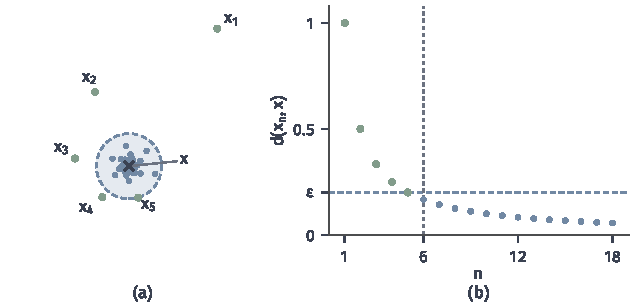
\includegraphics[width=108mm]{figures/04-spaces-measures-and-geometry/01-topology-and-metric/matplotlib/metric-sequence-tail/figure.pdf}
  \caption{点列$x_n=(\cos n/n,\sin n/n)$趋于原点$x$的两种读法，取$\varepsilon=1/5$。(a)平面上的点列，虚线圆是$B(x,\varepsilon)$，绿点是落在球外的前五项，蓝点是其后各项。(b)同一点列的距离数列$d(x_n,x)=1/n$，竖虚线处$N=6$，此后各点都在水平虚线$\varepsilon$之下。}
  \label{fig:metric-sequence-tail}
\end{BookInlineFigure}

判据的另外两个用法也值得记下。在乘积空间$(\mathbb R^m,\rho_\infty)$中，$\rho_\infty(\bm x_n,\bm x)\to0$当且仅当每个坐标的误差都趋于零，所以收敛就是逐坐标收敛；由于$\rho_1$与$\rho_\infty$诱导相同拓扑，换用$\rho_1$结论不变。

在离散度量$d_0$下，$d_0(x_n,x)$只取$0$和$1$，趋于零意味着从某项起恒为零。所以离散空间中的收敛点列，必须从某项起恒等于极限。

\subsection{收敛点列的性质}
\label{sec:metric-convergent-properties}

距离给出的第一个推论是极限唯一。若$x_n\to x$且$x_n\to y$，由三角不等式
\[
d(x,y)\leq d(x,x_n)+d(x_n,y)\to0,
\]
所以$d(x,y)=0$，由零距离判定得$x=y$。这里起作用的正是度量区分不同点的能力；第~\ref{sec:metric-pseudometric}小节的伪度量缺少这一条，常值点列可以同时趋于两个不同的点。

\begin{theorem}[收敛点列有界]
\label{thm:metric-convergent-bounded}
度量空间中的收敛点列，其全部项组成的集合是有界集。
\end{theorem}

\begin{proof}
设$x_n\to x$。取$N$使$n\geq N$时$d(x_n,x)<1$，前面只剩有限项，取它们的距离的最大值：
\[
r=1+\max\{d(x_1,x),\ldots,d(x_{N-1},x)\}
\]
（$N=1$时取$r=1$）。于是对每个$n$都有$d(x_n,x)<r$，全部项落在$B(x,r)$中。
\end{proof}

研究不收敛的点列时，常常从中挑出一部分。设$n_1<n_2<\cdots$是严格递增的正整数列，称$(x_{n_k})_{k\geq1}$为$(x_n)$的一个\term{子列}（subsequence）。严格递增保证$n_k\geq k$，所以$k\to\infty$时$n_k\to\infty$。

收敛点列的每个子列都收敛到同一个极限。设$x_n\to x$，对$\varepsilon>0$取$N$使$n\geq N$时$d(x_n,x)<\varepsilon$。当$k\geq N$时$n_k\geq N$，于是$d(x_{n_k},x)<\varepsilon$。

反方向不成立：一个点列有收敛的子列，不能推出它本身收敛。在$\mathbb R$中取$x_n=(-1)^n$，偶数项组成的子列恒为$1$，奇数项组成的子列恒为$-1$，各自收敛。若整列趋于某个$x$，两个子列都应趋于$x$，于是$x=1=-1$，矛盾。

整列收敛是比“存在收敛子列”强得多的要求，第~\ref{sec:metric-compactness}节的紧性判据只要求后者。

\subsection{闭包与闭集的序列判据}
\label{sec:metric-closure-sequences}

一个点离一个集合多近，可以用它到集合中各点距离的下确界来衡量。

\begin{definition}[点到集合的距离]
\label{def:metric-point-set-distance}
设$A\subseteq X$非空，$x\in X$。称
\begin{equation}
d(x,A)=\inf_{a\in A}d(x,a)
\label{eq:metric-point-set-distance}
\end{equation}
为$x$到$A$的\term{点到集合的距离}（distance from a point to a set）。
\end{definition}

在$\mathbb R$中取$A=(0,1)$，从定义算出
\[
d(2,A)=1,\qquad d(1,A)=0.
\]
第二个结果说明，下确界为零并不意味着$x\in A$，只说明$A$中有任意接近$x$的点。这正是闭包描述的情形。

\begin{theorem}[闭包的序列判据]
\label{thm:metric-closure-sequential}
设$A\subseteq X$非空，$x\in X$。以下三条等价：
\begin{enumerate}
\item $d(x,A)=0$；
\item $x$属于$A$的闭包$\overline A$；
\item 存在$A$中的点列$(a_n)$使$a_n\to x$。
\end{enumerate}
\end{theorem}

\begin{proof}
由(1)推(3)。对每个$n$，下确界为零意味着存在$a_n\in A$使$d(x,a_n)<1/n$，于是$a_n\to x$。

由(3)推(2)。$x$的每个邻域都包含某个$B(x,r)$，而$n$充分大时$a_n\in B(x,r)$，所以每个邻域都与$A$相交。

由(2)推(1)。对每个$n$，$B(x,1/n)$与$A$相交，取其中一点$a$，得$d(x,A)\leq d(x,a)<1/n$。$n$任意，所以$d(x,A)=0$。
\end{proof}

证明中由(1)推(3)的一步对每个$n$选出一个点，用的是可数个半径$1/n$，这正是度量空间每点有可数邻域基的用处。由(3)推(2)在任意拓扑空间中都成立，反方向则不然：第~\ref{chap:topological-spaces}章的余可数拓扑中，$\mathbb R\setminus\{0\}$的闭包是$\mathbb R$，却没有其中的点列收敛到$0$。

点到集合的距离本身也随$x$连续变化。对任意$a\in A$，由三角不等式
\[
d(x,A)\leq d(x,a)\leq d(x,y)+d(y,a).
\]
对$a$取下确界，得$d(x,A)\leq d(x,y)+d(y,A)$；交换$x,y$，又得到另一侧的不等式。合起来是
\begin{equation}
\lvert d(x,A)-d(y,A)\rvert\leq d(x,y).
\label{eq:metric-distance-to-set-lipschitz}
\end{equation}
因此闭包$\overline A=\{x:d(x,A)=0\}$可以看成一个连续函数的零点集，第~\ref{chap:metric-space-maps}章将从连续映射的角度回到这一点。

把定理~\ref{thm:metric-closure-sequential}用于两类特殊的集合，就得到稠密集和闭集的判据。$A$稠密是指$\overline A=X$，所以$A$在$X$中稠密，当且仅当$X$的每个点都是$A$中某个点列的极限。

$A$是闭集是指$\overline A=A$，所以$A$是闭集，当且仅当$A$中的点列只要在$X$中收敛，极限就属于$A$。

\begin{example}[序列判据的使用]
\label{ex:metric-sequential-criteria}
有理数在$\mathbb R$中稠密：对实数$x$，取它的十进制截断$q_n$（保留$n$位小数），则$\lvert x-q_n\rvert\leq10^{-n}$，$q_n\to x$。

集合$[0,1]$是闭集：若$a_n\in[0,1]$且$a_n\to x$，不等式在极限下保持，所以$0\leq x\leq1$。集合$(0,1]$不是$\mathbb R$的闭集：$1/n\in(0,1]$趋于$0\notin(0,1]$。

但若环境空间换成$X=(0,1]$，同一个点列在$X$中没有极限，$(0,1]$作为$X$自身仍是闭集。闭集的序列判据只要求保留环境中已经存在的极限；环境缺少某个极限点时，判据不对它提出要求。
\end{example}

环境本身是否缺少极限，正是下一节完备性要讨论的问题。
